% This is samplepaper.tex, a sample chapter demonstrating the
% LLNCS macro package for Springer Computer Science proceedings;
% Version 2.20 of 2017/10/04
%
%\documentclass[runningheads]{llncs}
\documentclass[conference]{IEEEtran}
%
\usepackage{graphicx}
% Used for displaying a sample figure. If possible, figure files should
% be included in EPS format.
%
% If you use the hyperref package, please uncomment the following line
% to display URLs in blue roman font according to Springer's eBook style:
% \renewcommand\UrlFont{\color{blue}\rmfamily}
\usepackage{verbatim}
\usepackage{color}
%\newcommand{\gl}[1]{\textcolor{red}{#1}}

\begin{document}
%
\title{The Evolving Passwords for WLAN Authentication with Location-based Physical Controls
}
%
%\titlerunning{Abbreviated paper title}
% If the paper title is too long for the running head, you can set
% an abbreviated paper title here
%

%
\maketitle              % typeset the header of the contribution
%

%本文没有带来安全性上的提高(如果硬认为有,那就是动态更新PSK)
%主要贡献点就是 可以动态更新更新PSK
%%可以就这点说明,PSK需要动态更新,否则由于传播,将导致PSK的大规模泄露;
%%%%--但本文中,只要泄露了中间一次PSK,是不是只要物理接近,就可以一直使用?
%物理位置,我不认为值得特别说明,是一个显然的事情,因为只有在物理位置接近时,才可以用WIFI

%\section{Abstract}
\begin{abstract}
In public areas such as company,libraries, coffee shops or hotels, WLANs is widely used because they are often free for users. Typically the administrators of the WLANs sets a password that is fixed during a period of time and any mobile devices can access the network by the WPA-PSK protocol if they get the password. The open communications environment and fixed password makes wireless transmissions more vulnerable to malicious attacks. The password is relatively simple  which has the risk of being guessed by the attacker. Meanwhile, as the password is unchanged, once the attackers or the unauthorized users get the password, they can access the network freely unless the password expires. For temporary visitors, fixed password makes them always have access permissions of the wireless network, which is obviously not conducive to the dynamic management of access rights.

 %However, none of the existing WLAN authentication methods well combine the above two goals.
 
This paper introduces a WLAN dynamic password scheme combined with physical access control, which can be applied to large-scale guest WLANs of large organizations. In this scheme, the WLAN password is automatically updated every specified interval without additional action by the administrator. Once the AP updates the password, mobile devices must update the password synchronously to access WLAN again. 
%A physical authentication factor is introduced to the password updating process. Users must pass the physical authentication and enter a specific location to get the physical authentication factor. Then mobile devices use the physical authentication factor to calculate the new password and continue accessing WLAN.
Because the password is updated periodically, this scheme can effectively prevent fake AP attacks,brute force attacks and revoke the access rights of visitors dynamically. We use some indexes to assessment the performance of our scheme, experiments show that the proposed scheme has little influence on system performance. Meanwhile, it can improve the experience of WLAN administrators and users, and improve the security of WLAN systems.
\end{abstract}
 

\begin{IEEEkeywords}
Dynamic Password, WLAN Access, Physical Authentication
\end{IEEEkeywords}
\section{Introduction}
\label{sec:Introduction}
Nowadays, WLAN has gained much more popularity than ever before with the popularity of mobile devices and mobile Internet because of its cheapness and fastness. We can now receive wireless signal almost everywhere such as in a park, on a bus, at home, or in workplace~\cite{gong2015advanced}. When we visit a new place, requiring for WLAN access often becomes one of the first things we do. Hence, it is of paramount importance to improve wireless communications security because more and more people are using wireless networks for online banking and personal emails, owing to the widespread use of smartphones~\cite{zou2016survey}. At the same time, there are two kinds of users joining such WLAN with different demands. The staff want a long-term WLAN access authorization while visitors only need to temporarily join WLAN, so  WLAN authentication becomes a problem.  It should achieve differential WLAN access control for both visitors and staff, and dynamic WLAN access control for different visitors. 


There are several solutions to settle above problems now, an  WLAN can be secured by the 802.11i protocol with pre-shared key mode(also known as WPA-PSK protocol)~\cite{Gu2011Research}. To provide higher security and more fine-grained access control, an organization can build a robust and secure  WLAN by the 802.11i protocol with 802.1X authentication server mode (also known as WPA-EAP protocol)~\cite{lashkari2009survey}. However, the most common authentication mechanism of a  WLAN is to deploy a web portal server equipped with WIFIDog. The web portal server can use various ways to authenticate users. 


One solution is to build an open WLAN. There is no authentication of this kind of WLAN, The WLAN is not protected by password, backward authentication server or any other approaches.It is the most convenient solution, but the disadvantage is also obvious. Any visitors can join WLAN freely including unauthorized users, more than that,this solution don't provide secure communication and encryption transmission~\cite{ Park2003WLAN}. Attackers will be able to intercept authorized users’ communication data, so users' private information may be revealed~\cite{Lamport1981Password}. 


Another solution is to build a relatively secure WLAN by the 802.11i protocol with pre-shared key mode(also known as WPA-PSK protocol)~\cite{macmichael2005auditing}. This password-based authentication mechanism~\cite{Burch2016Time} prevents unauthorized users who do not know the password accessing WLAN. If visitors want to join WLAN, they need to ask for password from administrators or authorized users first. However, this kind of authentication cannot prevent users who have known password joining WLAN as password usually stay unchanged for a long time. Thus, it cannot revoke visitors’ authorization of WLAN access when they leave. Besides, password is usually easy to guess, and a brute force attack is considered effective. If the password is compromised, there is no security for this kind of authentication. 


A more fine-grained but uncommon solution is to build a WLAN by the 802.11i protocol with 802.1X authentication server mode (also known as WPA-EAP protocol)~\cite{akhlaq2007comparative}. Administrators create accounts for every visitor, and probably set expiration time at the same time. When they leave, administrators delete their accounts to revoke their authorization. Users join WLAN with their own accounts during expiration time. But this kind of authentication adds a heavy burden on administrators especially when there are quite a few visitors coming and leaving everyday because everything relies on administrators. For convenience, administrators may create a single account for all visitors. All visitors share the same account which remains unchanged for a long time. Just like password-based authentication, it is hard for administrators to revoke authorization when visitors leave away. For educational institutions like universities, they have another choice - joining the Eduroam alliance and building a guest WLAN for visitors from other members in the alliance. Eduroam ~\cite{florio2005eduroam}provides wireless roaming for students, teachers, and researchers, enabling these people to join other educational institutions’ WLAN using accounts in their own institutions. So other educational institutions need not create accounts for these people. Eduroam helps WLAN reduce its burden in maintaining visitors’ accounts. But not all visitors are able to enjoy the wireless roaming service, administrators should also consider visitors not in the Eduroam alliance~\cite{Ó2007Deploying}. 


A portal server equipped with WiFiDog is widely used in guest WLAN~\cite{Lenczner2005Wireless}. Exactly speaking, it is a way of WLAN authorization rather than a way of WLAN authentication. Mobile devices should authenticate to APs first by the above mentioned ways. In most cases, the WLAN is open. That is, all users (authorized or unauthorized) are allowed to join WLAN. However, users cannot surf the Internet until they pass the authentication of the portal server. Once users connect to WLAN, they will be redirected to a login web page and required for login. There are several methods to login: 
\begin{itemize}
    \item Login by telephone number. Users type in their telephone numbers first. The portal server then will send a message carrying a verification code to the user’s telephone. Users then type in the verification code to login~\cite{Hallsteinsen2007Using}; 
    \item Login by wechat account. Users press the key of wechat login. This action will evoke the wechat application. In the wechat applicant users press the key of consent. Then users will be redirected back to the login page and achieve single sign-on; 
    \item Login by wechat friends. The process of this login method is just like the above. However, the login user is allowed to achieve single sign-on only if the his/her wechat account is the administrator’s wechat account;
     \item 	Login by inviters’ invitation. A QR code is displayed on the login page waiting for inviters (aka authorized users) scanning. Inviters scan the QR code to let invitees login to portal server;
     \item Login by username and password. Users type in their usernames and passwords at the login page to login.
\end{itemize}


Though there are so many authentication methods can be applied to portal server, there are still potential security risks on this kind of authentication. This kind of authentication does not provide extra security enhancement on WLAN transmission. In most cases, WLAN is open, all datas will be transmitted in plain text on WLAN. Besides, the former two authentication methods cannot filter users at all. All users including authorized or unauthorized can join WLAN freely. The last authentication method put heavy burden on administrators as it is a centralized solution.  

However, none of the existing solutions can realize the demand of guest WLAN - providing fine-grained access control and high security while not putting extra burden on users and administrators. For example, all users (authorized or unauthorized) can join an open guest WLAN. All messages transmitted on an open guest WLAN are in plaintext, and thus users’ private information may be revealed. Meanwhile, it is impossible to realize user access control for an open WLAN. As for password based authentication, though it can prevent unauthorized users joining WLAN, it is hard to revoke visitors’ authorization of WLAN access once they are told the password. This kind of authentication is not secure enough as passwords are guessable. Although the 802.1X authentication server based authentication can provide very fine-grained access control for each user~\cite{ Afia2007Comparative}. However, it introduces a heavy burden on administrators as all users rely on administrators operation on user account. Authenticating by a web portal server equipped by WIFIDog can indeed realize various demand of WLAN access control. However, this kind of authentication cannot provide any extra confidentiality and integrity protection for transmitted data. Data security still relies on the base authentication mechanism, but it is common that this kind of authentication is deployed on an open WLAN which means there is no base authentication mechanism. 


In this paper, we want to combine fine-grained access control, convenience and security for WLAN. Our goal is to achieve differential WLAN access control for visitors and staff - staff can always join WLAN while visitors can only join WLAN during their visit, and dynamic WLAN access authorization for visitors - granting when they come and revoking when they leave. Meanwhile, we do not want to put extra burden on administrators. To achieve this goal, we proposed a location-based evolving passwords scheme for WLAN authentication. WLAN passwords will automatically evolve at regular intervals. Administrators can adjust the update interval whenever needed. If passwords evolve, only authorized users can get new passwords and continue to join WLAN. This means, unauthorized users knowing old passwords will be filtered out and cannot connect to WLAN any longer. To prevent unauthorized users renewing passwords, we introduced physical access control into passwords evolving process. A random number called physical parameter is used to renewing passwords. A specific device generates physical parameters and broadcasts them to a specific location protected by a physical access control system. Thus, users can only obtain physical parameters in constrained locations. In order to obtain physical parameters and renew passwords, authorized users must pass physical access control systems. Visitors who have finished their visit will not be able to get the physical parameter. Thus, they cannot get new passwords and join WLAN, even though they may still receive wireless signal. Most important, the new dynamic password scheme will not put extra burdens on authorized users and administrators. Authorized users can still get passwords from administrators or authorized users and join WLAN as usual. Passwords will evolve automatically without participation of administrators and authorized users. 


We have implemented the proposed scheme. An authorized mobile device can successfully extract physical parameters, calculate new passwords, and authenticate to APs before and after passwords evolving. There is almost no connection delay compared with the static password scheme. What authorized users and administrators need to do is just as usual. 


Contributions:
We proposed a location-based evolving passwords scheme for WLAN authentication, providing fine-grained access control for different users while not putting extra burden on administrators and authorized users. 
%动态权限管理
We combine physical authentication and WLAN authentication: whether users can connect to WLAN depends on whether they can pass physical access control systems. 
%By this way, we achieved dynamic authorization for visitors: %when they come, they need to request for WLAN access %authorization; when they leave, their authorization will be %revoked in time. 
%一般员工WIFI和访客WIFI是分开的,,,,
Regular staff can always pass physical access controls and update passwords. As for visitors, once they ended their visit, they would not pass physical access controls and so they would not get new passwords even though they can still receive wireless signal, so their authorization will be revoked in time
%抵抗穷举攻击和假冒AP攻击
What’s more, we enhanced the security of the password-based WLAN authentication. WLAN passwords are automatically changed from time to time. The password update interval is short enough to avoid brute force attacks and fake AP attacks. Even if an attacker gets a password, he/she will be filtered out when passwords evolve minimizing negative influences of a successful attack. For the fake AP attack, the fake AP can induce the user to access the insecure wireless network by setting the same password. If the password  update regularly,this attack is also invalid.
%大型部署
In our proposed scheme, only one master AP is located in a controlled environment, which produces and distributes physical parameters. Slave aps can be located outside of a physically controlled environment, this mode of operation is suitable for large-scale guest WLANs of large organizations.

\section{Assumptions and threat model}
\subsection{Assumptions}
We have the following two assumptions for our proposed scheme. 
Unreachable location for unauthorized users. In the proposed scheme, physical parameters can only be obtained in a constrained location. Considering a big building, there shall be one or more places protected by physical access controls such as entrance guard in the building. Only when users show their access card to the entrance guard, swipe their access guard, type in their password, or unlock the door using a key, can they get into such places. For authorized users’ convenience, it would be better if authorized users will frequently pass by such places.  


Authorized users willing to install an application. It is necessary for authorized users to install an application on their mobile devices for extracting physical parameters and updating passwords. The application is small enough. We assume authorized users are willing to download and install it using their mobile data traffic. 

\subsection{Threat model}
No attacks except for brute force attack. We adopt the 802.11i protocol with pre-shared key mode to achieve the authentication between APs and mobile devices. However, the pre-shared key will automatically evolves~\cite{Pinto2016Hash} from time to time. There are several kinds of attacks targeting at the 802.11i protocol with pre-shared key mode. Brute force attack is a very common form as passphrases are easy to guess and stay unchanged for a long time. If attackers successfully guess out passphrases, they are able to join WLAN freely. We assume attackers can conduct a brute force attack on the evolving passwords scheme to get pre-shared keys. 
Except for brute force attack, we assume there is no other attacks on the proposed scheme. We assume authorized users will not install malicious applications stealing passwords. We assume passwords will be distributed in a secure channel and attackers cannot eavesdrop. We also assume the 802.11i protocol is secure enough to prevent attackers from connecting to APs without passphrases and pre-shared keys.


\section{System Overview}
\label{sec:systemoverview}
We introduced a location based evolving passwords scheme into the 802.11i protocol with pre-shared key mode to provide fine-grained access control and high security for WLAN. But just as significantly, introducing of evolving passwords scheme will not put extra burdens on administrators and users. To join WLAN, mobile devices must share the same password with APs at the same time, or they cannot pass APs’ authentication. However, we make passwords evolve at short intervals. A long random number is used to generate the updated password. It is called physical parameter because it can only be obtained in a constrained location protected by physical access controls for mobile devices. Once APs update their passwords, mobile devices have to  synchronize their own passwords with APs’ to join WLAN.


As is shown in Figure~\ref{fig:Overview of the WLAN System with Location Related Dynamic Password}, the location based passwords evolving system consists of three parts: a special device called physical generator which generate and broadcast physical parameters at regular intervals, one or more APs whose passwords evolve automatically at set intervals, and one or more mobile devices which are able to synchronize passwords with APs automatically when necessary and possible. 

\begin{figure}
    \centering
    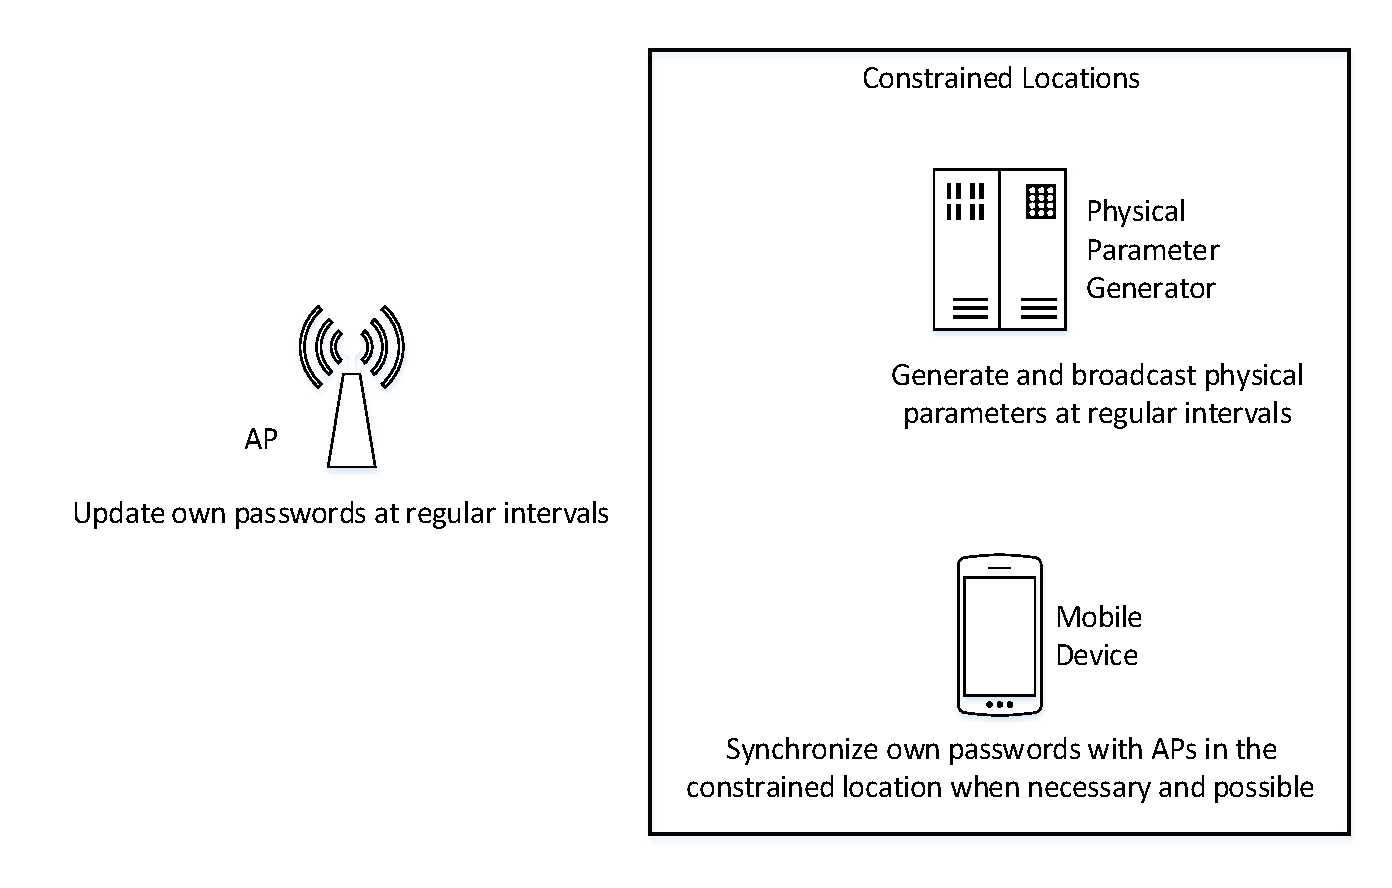
\includegraphics[width=0.5\textwidth]{pic/1.pdf}
    \caption{The WLAN System with Location Related Dynamic Password.}
    \label{fig:Overview of the WLAN System with Location Related Dynamic Password}
\end{figure}

 
\begin{itemize}
    \item the physical parameter generator will generate new physical parameters and broadcasts them to a constrained location protected by physical access controls; 
    \item APs get new physical parameters though a secure channel and update their own passwords; 
    \item  mobile devices can get new physical parameters if users pass physical access controls and update their own passwords by the same way with APs. 
\end{itemize}
	
	
APs’ initial passwords are set by administrators while mobile devices’ initial passwords are obtained through an out-of-band way. When passwords evolves, both APs and mobile devices can get the same new passwords on the basis of the same old passwords and physical parameters. The passwords evolving process is simple. The passwords evolving process of each AP and each mobile devices is independent of each other. 

\section{Large Organization Scenario}
\label{sec:large}

The evolving passwords scheme with location-based physical access controls can be deployed by a large organization in a big building with many visitors coming and leaving everyday. Considering a wide WLAN in a big building, there shall be several APs with their wireless signal covering the whole building. We assign one of such APs as the physical parameter generator and call it master AP. Physical parameters are broadcast though master AP’s wireless signal. By this way, mobile devices can only get physical parameters in the constrained location. Thus, only users who pass physical access controls and enter the constrained location can get physical parameters and synchronize their passwords with APs after passwords evolving. 	

\subsection{General Framework}
A WLAN system deployed with the proposed evolving passwords scheme consists of three parts: 
\begin{itemize}
    \item a master AP which can update its own password independently,
    \item several slave APs which can update their own passwords by interaction with the master AP, 
    \item many mobile devices which can connect to APs and automatically synchronize their own passwords with APs’.
\end{itemize}

The passwords evolving procedure can be divided into four: 
\begin{itemize}
    \item initial password setup and distribution,
    \item password update interval setup, 
    \item physical parameter generation and broadcast,
    \item password update of APs and mobile devices. 
\end{itemize}

The former two procedures will be executed only once in the initialization phase when the procedure starts, while the latter procedures will be repeatedly executed in the passwords evolving phase at regular intervals. 


In the initialization phrase, an initial password and an update interval is set by administrators and stored in configuration files on the master AP. An authenticator on the master AP reads the initial password and the update interval from configuration files when launched. For slave APs, it is unnecessary for administrators to set initial passwords for every slave AP. Instead, administrators specify the address of the master AP for slave APs, so authenticators on slave APs could acquire the current password from the master AP by a safe way. As for mobile devices,  initial passwords are obtained through an out-of-band way and the latest password will be stored in configuration files. 

After initialization, all APs will automatically update their passwords at regular intervals preset by administrators, while mobile devices will automatically synchronize their passwords with APs and join WLAN if possible. The evolving passwords phrase of every part is shown as graph 2. 

\begin{figure}
    \centering
    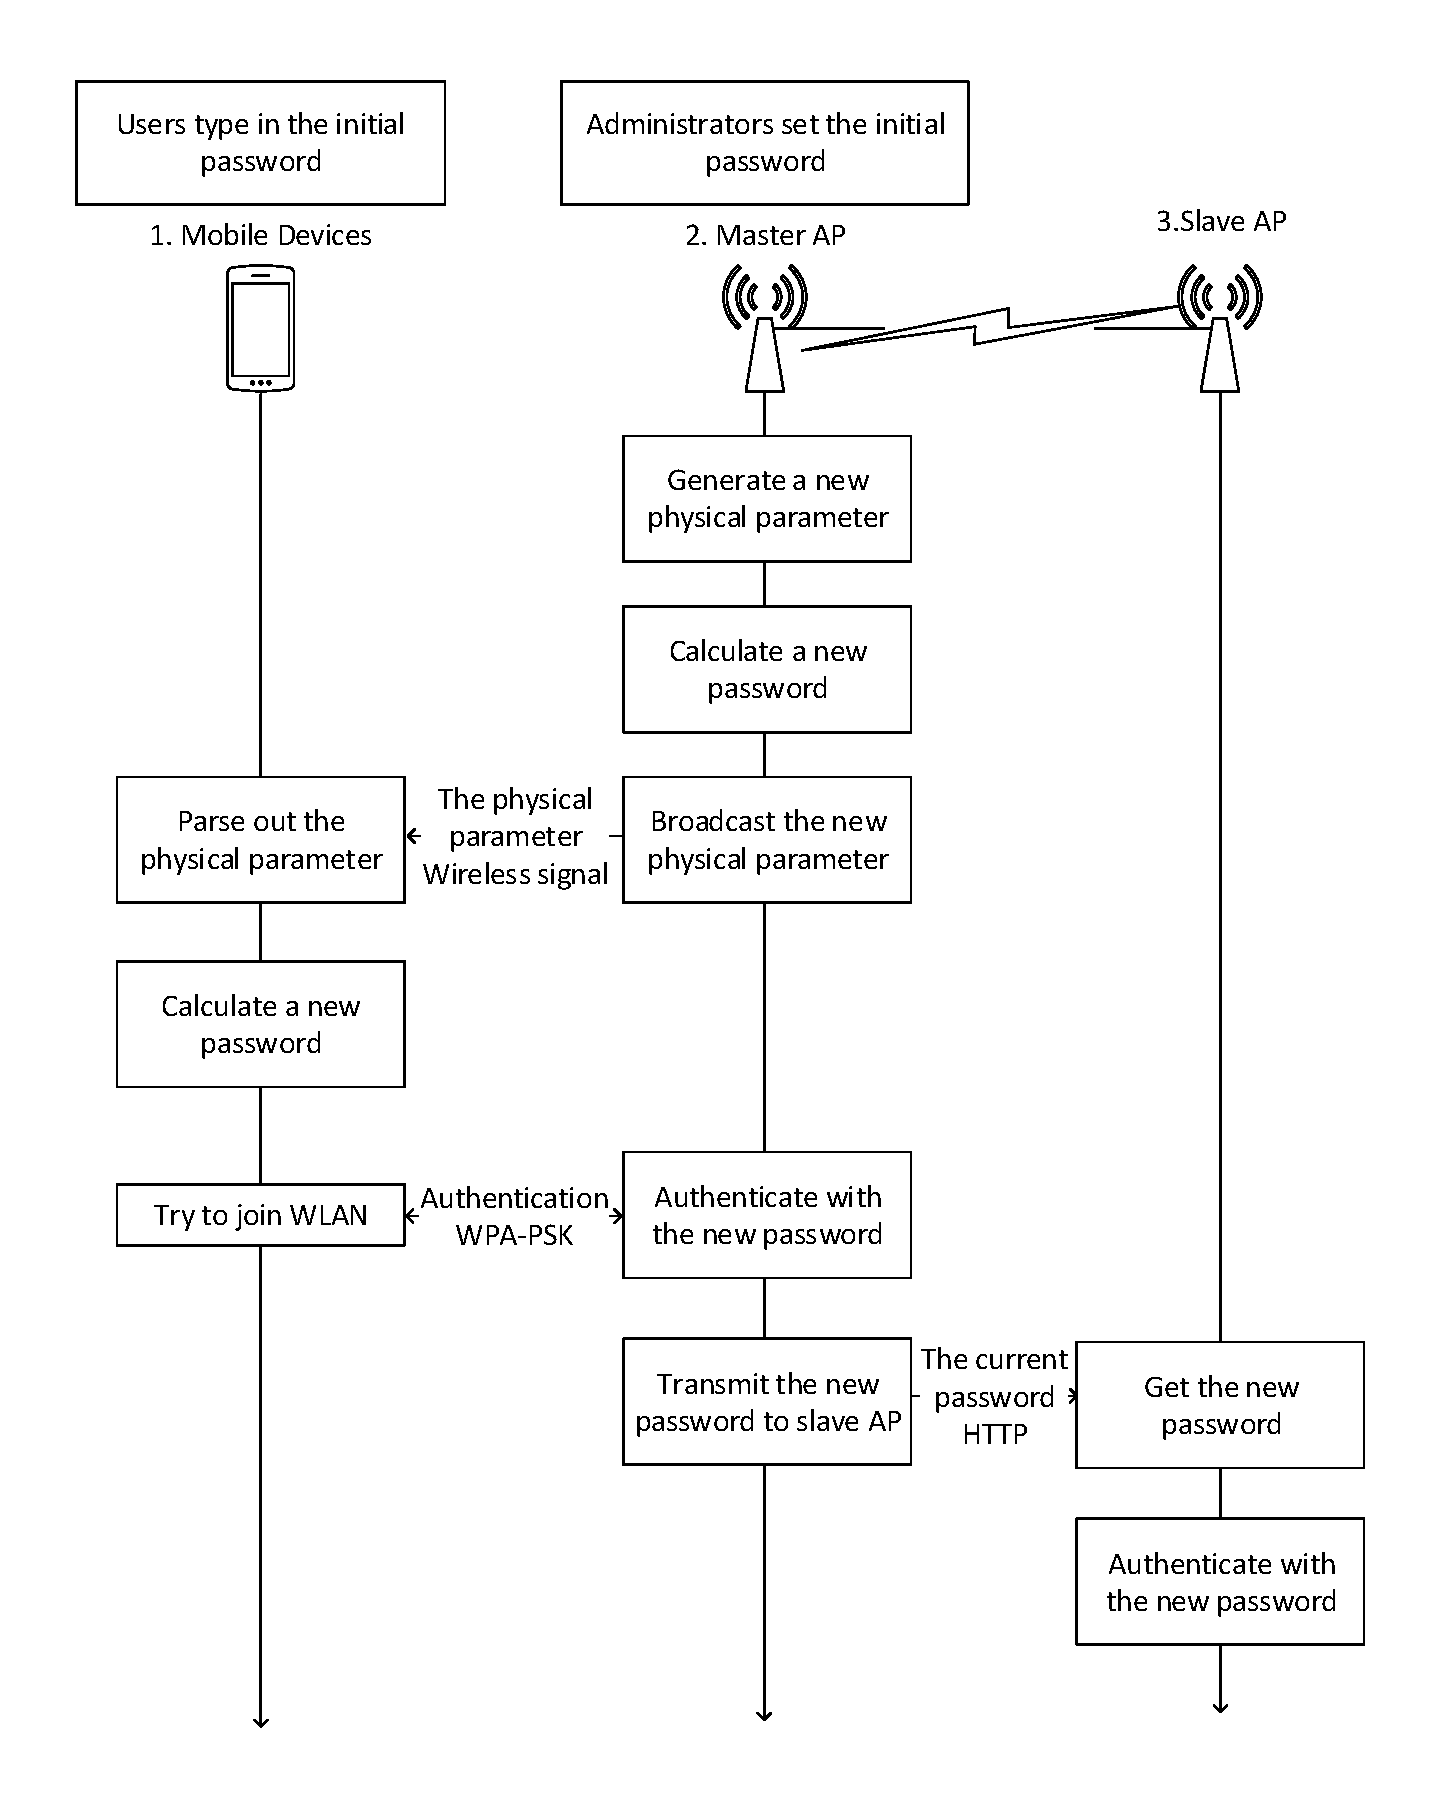
\includegraphics[width=0.5\textwidth]{pic/2.pdf}
    \caption{The Work Flow of the WLAN System with Location Related Dynamic Passwordd.}
    \label{fig:xxx}
\end{figure}


For the master AP, it need to complete the following works: 
\begin{itemize}
    \item Generate a long random number as a new physical parameter; 
    \item Calculate a new password using the old password and the new physical parameter; 
    \item Broadcast the new physical parameter to the constrained location protected by physical access controls; 
    \item Transmit the new password to slave APs securely. 
    \item Authenticate mobile devices using the new password; 
\end{itemize}
	

As for slave APs, they need to complete the following works: 
\begin{itemize}
    \item Require a new password from the master securely; 
    \item Authenticate mobile devices with the new password. 
\end{itemize}
	
As for mobile devices, they need to complete the following works: 
\begin{itemize}
    \item Capture WLAN signal and parse out the physical parameter from it; 
    \item Calculate out a new password by the same way with the master AP; 
    \item Try to join WLAN with the new password; 
    \item If joining successfully, accept the new password;
    \item If not, reject the new password and roll back.  After that, mobile devices can continuously join WLAN before next time passwords evolving. 
\end{itemize}

\subsection{Specific Detail}
The proposed evolving passwords system has some details which are worth specifying. 

\subsubsection{Password Format}
Mobile devices can join WLAN by the 802.11i protocol if they share the same pre-shared key with APs. In the 802.11i protocol, there are two password related concepts: passphrase and pre-shared key. The passphrase is a short string usually containing 8-20 characters which is easy to remember and type. Usually the passphrase is used to generate a 32 byte pre-shared key using a pseudo random generation algorithm. Then the pre-shared key will be used in a 4-way handshake for authentication between mobile devices and APs. 


In the proposed evolving passwords scheme, the password is the same as the pre-shared key with a length of 32 bytes which is the result of a secure hash algorithm such as SM3, SHA256. If the hash result is longer than 32 bytes,the first 32 byte of the result is used as the pre-shared key. The pre-shared key is too long to type in, we use the QR code to distribute it. The pre-shared key can be displayed on the screen or printed on the paper in the form of QR code. Authorized users can get the current password by scanning the QR code. As most of mobile devices are equipped with camera, it will not be a big problem for authorized users. 

\subsubsection{Password Update Interval}
In the initialization phrase, an update interval is set by administrators and it can be adjusted according to practical circumstances. In general, administrators can set a slightly longer update interval. However, when something important happens, they can shorten it for security considerations. This feature can be achieved as follows. 

All passwords have their expiry time, every time the master AP updates its password, its expiry time is increased by the the update interval. When slave APs require the current password, its expiry time will be responded at the same time. So slave APs know when the current password will be expired and when to request for a newer password from the master AP. 

If administrators want to change the update interval, he/she could modify the update interval and restart the authenticator on the master AP. When the authenticator restarts, it will continue using the current password until it is expired. However, when the current password is expired, the master AP will apply the new update interval. For slave APs, they get the expire time from the master AP, so modifying the update interval will not influence the update procedure of all APs in WLAN. 


However, if administrators do not want to wait until the current password expired, they have to modify the expiry time of the current password, and then restart all authenticators on the master AP and slave APs. By this way, the current password is forced to be expired in advance. 

\subsubsection{Broadcast Method of Physical} Parameters
At the process of the passwords evolving phrase, an physical parameter is generated and broadcast by the master AP. Physical parameters can be broadcast by the master AP’s wireless signal as it is limited in a constrained location. The beacon frame can be used to broadcast physical parameters. Usually, an AP will broadcast beacon frames at short intervals to announce existing of a special WLAN. There is a vendor specific field in the beacon frame which can carry custom data. The data structure of the vendor specific field consists of three parts: tag, length, and value. Custom data is carried in the value part. Different kinds of custom data is distinguished by the first 3 bytes called OUI. The next byte of OUI is OUI type. And the structure of the subsequent data depends on the concrete type of custom data, aka, OUI. The WLAN system can use a non-conflict OUI specially for physical parameter transmission. When mobile devices capture a beacon frame with a specific SSID, they can parse out the physical parameter in the vendor specific according to the predetermined OUI and OUI type. 

\subsubsection{Variable Broadcast Number of Physical Parameters} 
The master AP can broadcast one or more physical parameters to adjust the frequency of authorized users entering the constrained location. If the master AP update one password and broadcast one physical parameter , authorized users must enter the constrained location in every update period. If an authorized user has not entered the constrained location in one update period, he/she would never calculate out subsequent passwords. Even if he/she enters the constrained location in the next update period, he/she cannot calculate out the current password as he/she does not know the previous password which is necessary for calculating the current password. However, if the master AP broadcasts two physical parameters aka current and next physical parameter, it does not matter if an authorized user does not enter the constrained location in the next update period after he/she enters the constrained location in the current update period. Using the two physical parameters, he/she are able to calculate out the current and next password. When he/she enters the constrained location in the next of the next update period, he/she could still calculate out the password. If the master AP broadcasts more physical parameters, the time span authorized users entering the constrained location can be even longer. 


This feature can be applied to such a situation. Usually, the staff is required to be on duty every weekday. So the update interval can be set to one day. However, the staff may not go to work at the weekend. If the master AP still broadcasts one physical parameter on Friday, the staff cannot join WLAN on Monday. For the staff successfully joining WLAN on Monday, the master AP should generates and broadcasts three physical parameters on Friday. 

\subsubsection{Passwords Evolving Formula}
Once the master AP generates a new physical parameter, it calculates a new password with the old password and the new physical parameter. Let P[i - 1] as the old password, O[i] as the new physical parameter, the new password P[i] can be calculated out as follows: 
P[i] = Truncate(Hash(P[i - 1] XOR O[i]))\cite{m2005hotp}\cite{Liu2014An}. 
The hash algorithm can be SM2, SHA-256, and the like. As mentioned above, the password is a 32 byte number, but the hash value may be longer than 32 bytes. In this case, we can truncate the first 32 bytes of the hash value as the new password. 



\subsubsection{Password Transmission Channel between the Master AP and Slave APs} 
In the initialization phrase, slave APs should request for the initial password from the master AP. When the current password is expired, slave APs should request for a new password from the master AP. The password should be transmitted from the master AP to slave APs though a secure channel. For example, administrators can establish dedicated links for transmitting passwords between the master AP and slave APs. For another example, the above information can be transmitted through a common LAN. Though such LAN is insecure as it is connected with WLAN and Internet, the master AP can secure it by encrypting and adding a message authentication code before transmitting passwords, ensuring that only the master AP and slave APs share secret keys. It is also a proper way to establish a mutual authenticated TLS tunnel between the master AP and slave APs on LAN and transmit passwords in the TLS tunnel. 


\subsubsection{Password Synchronization between the Master AP and Slave APs}
The system time of slave APs may be later than that of the master AP. If so, there may be an out of sync of password update between the master AP and slave APs. That is, the master AP has updated passwords, but slave APs still use old passwords as it thinks old passwords have not been expired yet. To achieve a near-zero time delay between the master AP and slave APs, all APs should regularly adjust the system time from the same time server. Besides, slave APs could request a new password slightly earlier than the expiry time of the current password. If there is a long time delay between an slave AP and the master AP, mobile devices may not be able to connect to slave APs when they have once received a beacon frame from the master AP and already updated their own passwords. 



\subsubsection{Passwords Synchronization between APs and Mobile Devices}
If all APs update their own passwords, only mobile devices update their own passwords synchronously could they join WLAN again. Considering the update interval can be adjusted by administrators on demand, it becomes a problem how to inform mobile devices whether passwords evolve and how many times passwords have been evolved from mobile devices getting their initial passwords or updating their passwords last time. To solve this problem, we assign a serial number for the password. The serial number starts with zero and increases by one after passwords evolving. APs broadcast the serial number of the password they currently use to inform mobile devices whether they need to update their own passwords. Serial numbers can be broadcast through the beacon frame using the vendor specific field like physical parameters. They can have the same OUI but different OUI type compared with physical numbers. 


When mobile devices get the current password from administrators or other authorized users, its serial number is same. Mobile devices regularly capture and parse beacon frames. Once capturing frames with a specific SSID, mobile devices will parse out the serial number, and determines whether they share the same password with APs by comparing the two serial numbers. If the serial numbers of APs’ passwords is the same as that of their own passwords, it means they share the same password with APs and can join WLAN using the old passwords. If the serial number of APs’ passwords is greater by one than that of their own passwords, mobile devices can update their own passwords if they can get the current physical parameter. If else, mobile devices cannot update their own passwords to the current time. The system time of APs and mobile devices may also be different. However, it is not a big deal. Mobile devices use the serial number to determine whether they can synchronize their passwords with APs. The system time of mobile devices does not participate in the password update process. 


\subsubsection{Verification of Physical Parameters by Mobile Devices}
If mobile devices successfully parse out a physical parameters from a beacon frame, they calculate a temporary new password without updating their own passwords because the physical parameter may be wrong. Then it tries to join WLAN using the temporary new password. If it successfully connect to APs, it means the temporary new password is right. Until then, mobile devices could update their own passwords. If mobile devices fail to connect to APs, they should clear the temporary new password and wait for another physical parameter. 


\subsubsection{Consideration of an Unexpected or Planned Restart}
Once calculating out a new password, the master AP should store the new physical parameter and the new password with its expiry time into configuration files in case of an unexpected or planned restart. By this way, even if the master AP experiences an unexpected or planned restart, it still could get the newest physical parameter and the newest password. Therefore, it could continue broadcasting the newest physical parameter, use the newest password to authenticate mobile devices.


When the master AP restarts, the password in configuration files may have been expired. The master AP determines whether such password is expired by getting the current time and comparing it with the expiry time of the password. If the current time exceed the expiry time of the password, it should update the password to the current time. 


Mobile devices have a similar situation with the master AP, and they should also update configuration files when their passwords are updated. However, An unexpected or planned restart will not influence slave APs because they get the newest password from the master AP when they start. 


\section{Implementation}
If implemented properly, the WLAN system will run as expected. All APs in the WLAN will update passwords simultaneously and regularly. Mobile devices get current passwords through an out-of-band channel and join WLAN. Once the WLAN password is updated, mobile devices have to update their own passwords in order to join WLAN again. If mobile devices can capture the beacon frame of the master AP and parse out the physical parameter, they can calculate out the new password and successfully join WLAN. If not, they cannot connect to the WLAN but can inform users to pass the physical access control and get into the specific location to get the physical parameter and calculate the new password. However, if the WLAN password have been updated for more than once, mobile devices can do nothing but inform users that they cannot join WLAN again. 


We have implemented a WLAN system deployed with the proposed evolving passwords mechanism and evaluated the influence of it. We have evaluated the following indexes. 


\subsection{Connection Delay of Mobile Devices}
Connection delay of mobile devices means the time span from mobile devices receiving wireless signal to successfully joining WLAN. As mentioned above, mobile devices may use their own current passwords to join WLAN, or update their passwords and use new passwords to join WLAN. We have tested all of the above cases. We have also tested the connection delay of static passwords mechanism for comparison. Test results shows as below: 

\begin{table}[]
    \centering
    \begin{tabular}{|c|c|c|c|}
        \hline
         {Static } & {Without Password } & {With Password } &{Unable to }
         \\
        
         {Passwords} & {Update} & {Update} &{Join in}\\
         
         \hline
         {594.421ms}& {600.694ms} & {630.052ms} & {0.091ms} 
         \\
         \hline
    \end{tabular}
    \caption{Test Results of Connection Delay of Mobile Devices.}
    \label{tbl:connDelay}
\end{table}

Test results show that password update has little influence on mobile devices connecting to WLAN. 

\subsection{Reconnection Delay of Mobile Devices}
Reconnection delay of mobile devices means the time span from mobile devices losing connection of APs to reconnecting to APs. In our implementation, when getting new passwords, APs will restart to make new passwords come into force which means they will disconnect all mobile devices’ connections. Therefore, mobile devices need to reconnect to APs again. After restarting, APs will broadcast de-authenticate frames to all connected mobile devices. Then mobile devices will re-scan wireless signal. A separate program periodically query scanning results and parse serial numbers and physical parameters from scanning results. When it finds APs have updated their passwords and parses out new physical parameters, it will update mobile devices’ passwords and force mobile devices to reconnect to APs using new passwords. If mobile devices successfully reconnect to APs, the program will update mobile devices’ passwords. The reconnection delay is subject to query interval and shows as below: 

\begin{figure}
    \centering
    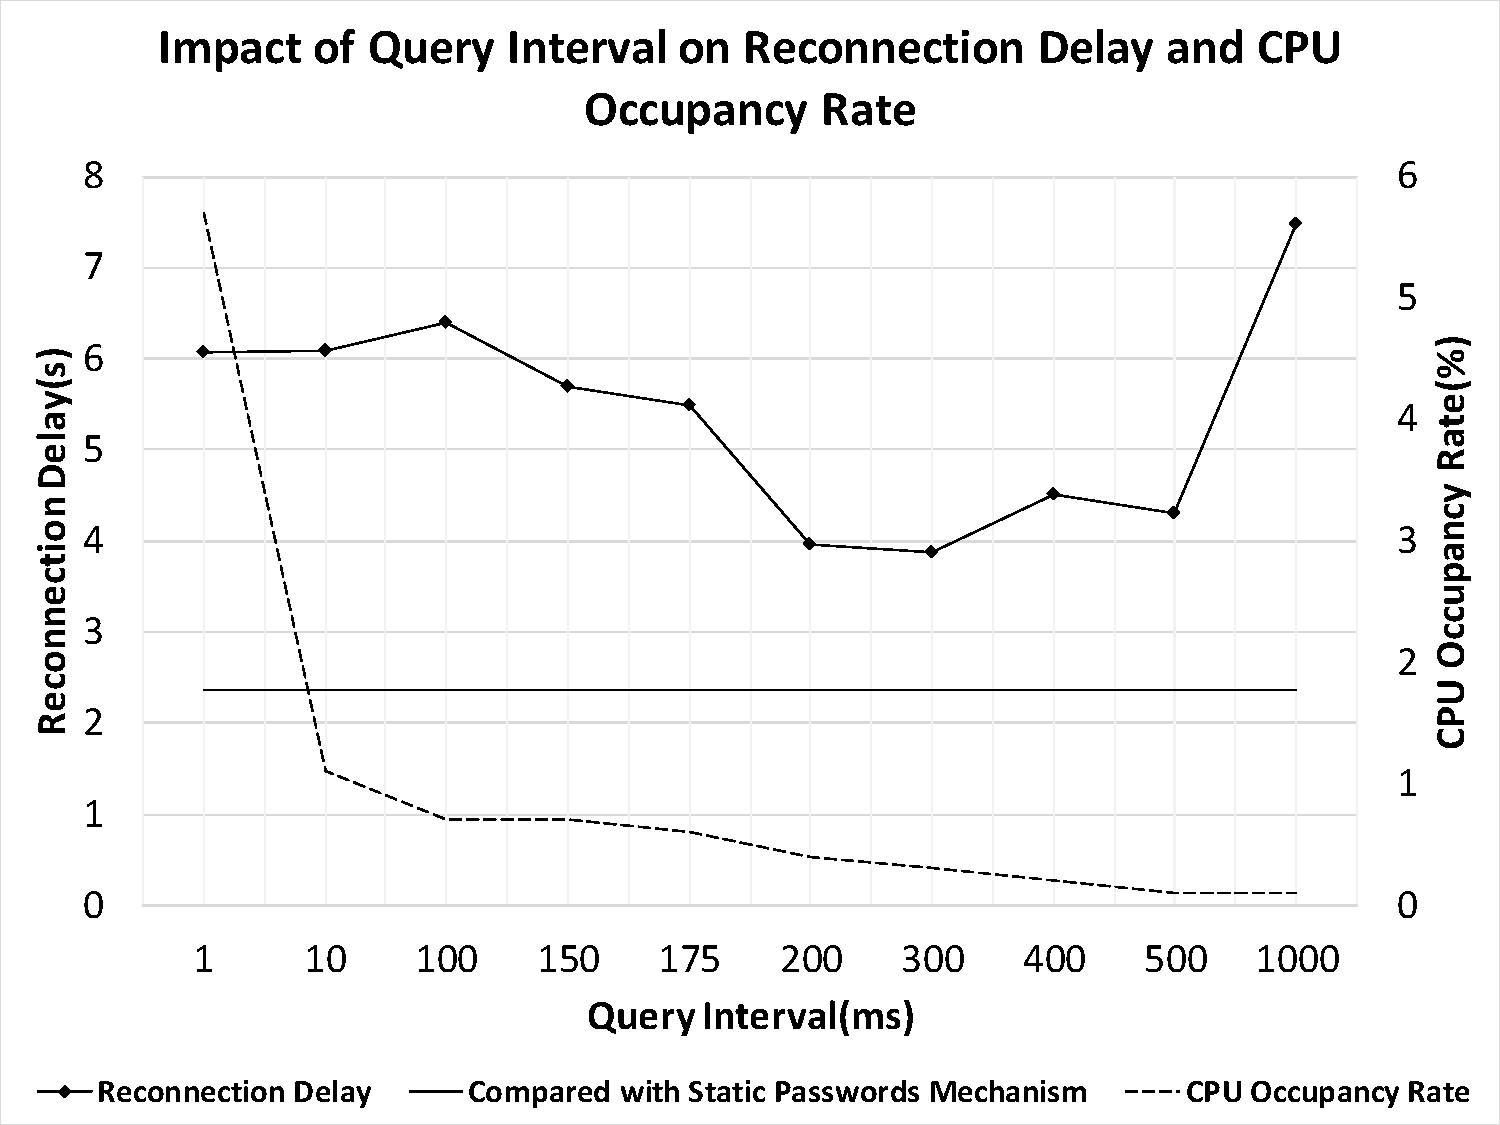
\includegraphics[width=0.5\textwidth]{pic/3.pdf}
    \caption{Impact of Query Interval on Reconnection Delay and CPU Occupancy Rate.}
    \label{fig:exp1}
\end{figure}




According to our analysis, the bottleneck is re-scanning wireless signal. Scanning will last for about 1.5 seconds while it may happens for more than once. It should be noticed that there is almost no influence on memory occupation whatever the query interval is.

\subsection{Update Delay of Slave APs}
Update delay of slave APs means the time gap between the master and slave APs update their own passwords separately. As mentioned above, the master AP update its passwords earlier than the slave APs. If the slave APs update their passwords much later than the master AP, it may cause problems on users when users move from wireless signal coverage of the master AP to wireless signal coverage of the slave APs. When users are under wireless signal coverage of the master AP and the master AP update its passwords, their mobile devices will update their passwords, too. However, when users move to the wireless signal coverage of the slave APs, they will be rejected to join WLAN because their mobile devices do not share the same password with the slave APs because the slave AP have not updated their passwords yet. It would be better if the update delay of slave APs can be as short as possible. If so, users can get a seamless experience when handover from one AP to another. When updating password, the slave APs request for a new password over and over again until a new password responded. The roll polling frequency influences the update delay of slave APs. A more frequent roll polling will shorten the update delay. However, it will also occupy a lot of system resources. We tested the influence of roll polling frequency. Test results shows as below: 


\begin{figure}
    \centering
    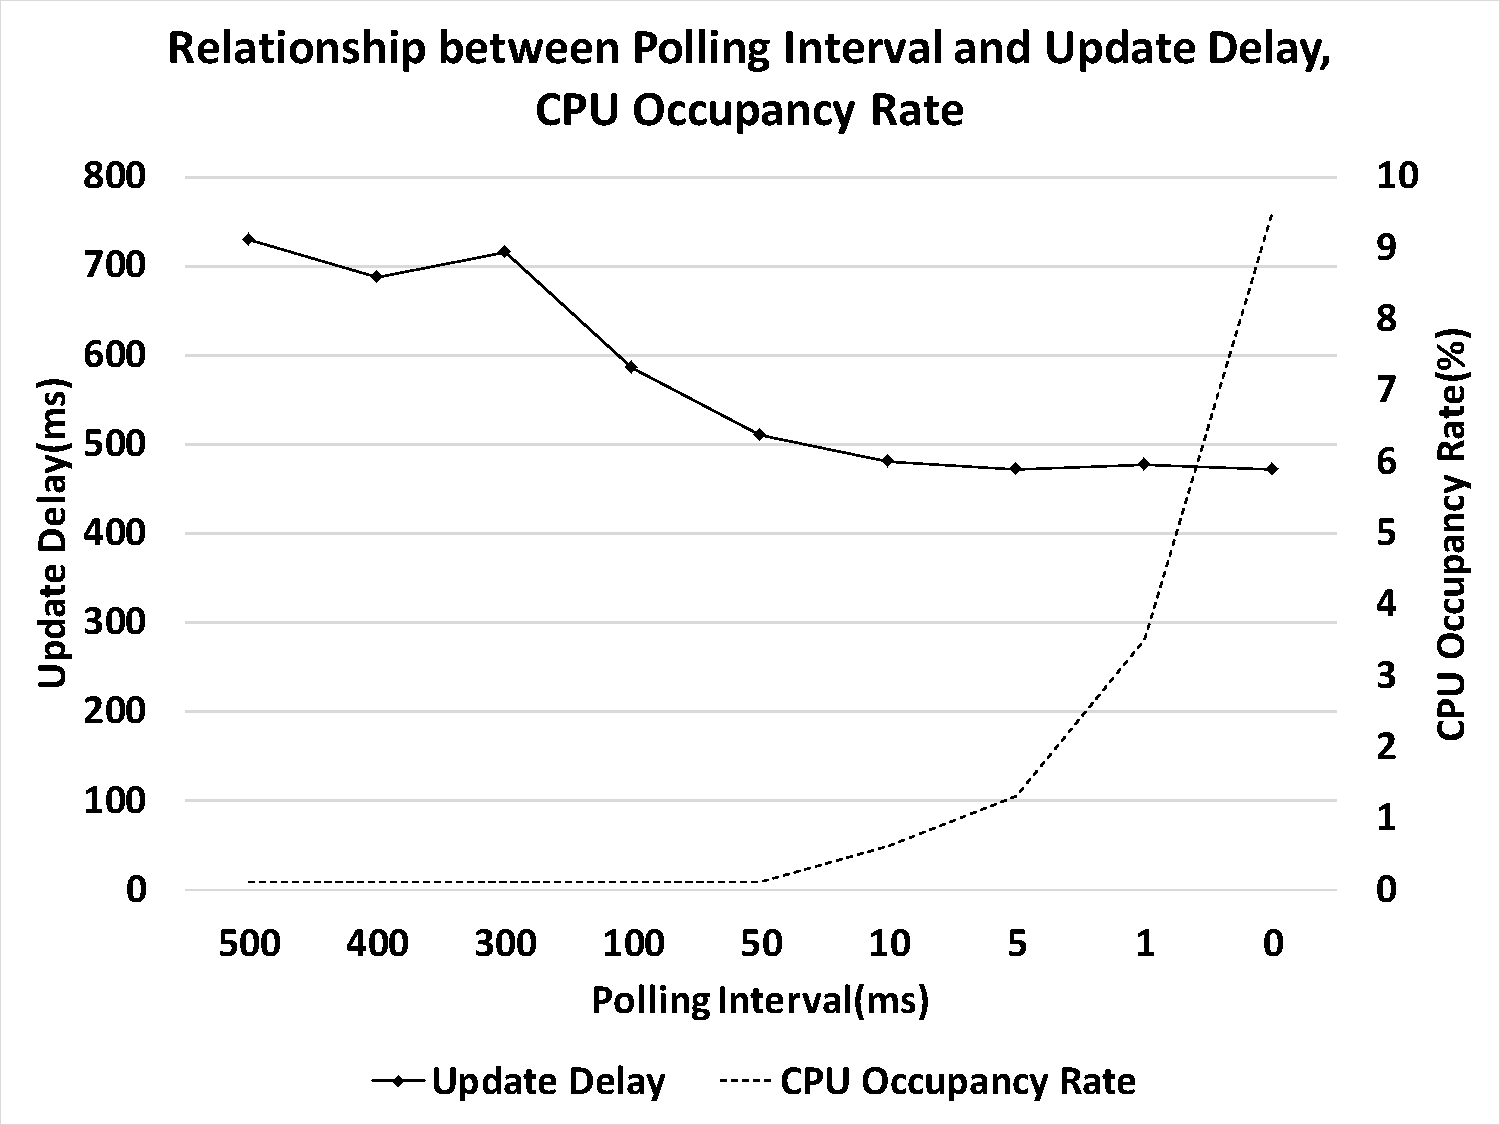
\includegraphics[width=0.5\textwidth]{pic/4.pdf}
    \caption{Relationship between Polling Interval and Update Delay, CPU Occupancy Rate.}
    \label{fig:exp2}
\end{figure}

It should be noticed that there is almost no influence on memory occupation and network flow when requesting new passwords from the master AP whatever the roll polling frequency is. If set properly, all APs will update their own passwords in a short enough delay without occupying too much system resource. 

\section{Security Analysis}
WLAN authentication is the foundation of WLAN security. The 802.11i protocol defines how to complete authentication and encrypt data before transmission. It can be run in two modes: pre-shared key based mode(also known as WPA-PSK) and 802.1X authentication server based mode(also known as WPA-EAP). For both modes, the authenticator and the supplicant should share a secret called PMK. For pre-shared key based mode, the PMK is derived from a pre-shared key, while the pre-shared key is derived form a passphrase. The passphrase is a short string usually containing 8-20 characters which is easy to remember and guess such as name, birthday or telephone. Administrators set passphrase for APs and tell it to authorized users. Authorized users type the passphrase into mobile devices. And then the authenticator and the supplicant will share the same PMK. For 802.1X authentication server mode, an 802.1X authentication server, usually a RADIUS server, is needed. The PMK is generated from a TLS negotiation between the authentication server and the supplicant and than the authentication server securely transport it to the authenticator. This mode is considered more secure as the TLS protocol is considered secure while the passphrase is vulnerable. Once the authenticator and the supplicant share the PMK, a 4-way handshake will be proceeded. We have observed that though there are many attacks aimed at the 4-way handshake, and some attacks are extremely critical, we can avoid all known exploits if deployed properly. So the 4-way handshake is still considered secure~\cite{Liu2010Survey} . After the 4-way handshake, the authenticator and the supplicant share a temporary secret key. They will use it to encrypt and decrypt communication data. 


In summary, the WPA-EAP protocol is still considered secure while the WPA-PSK protocol exists some security concerns. The short board of WPA-PSK protocol is the passphrase as the passphrase is easy to guess and remain unchanged for a long time. Once attackers get the passphrase, there is no security for the WPA-PSK protocol. Attackers will also be able to join the WLAN degrading authorized users’ online experience, get authorized users’ private information, or set up a fishing AP cheating authorized users connecting and transporting data to it. A brute force attack is considered realistic to obtain passphrase. Attackers can try all potential passphrases until finding the right one. Nevertheless, it may take much time for attackers to successfully implement an a brute force attack. However, the brute force attack can be accelerated with the help of cloud-computing, GPU, distributed algorithm, and the like. To improve the security of the passphrase-based WPA-PSK protocol, WLAN administrators should set complex passphrase which is hard to guess. They should change passphrases frequently and distribute new passphrases to authorized users. It will obviously increase the burden of both administrators and authorized users and is impractical for large WLAN. Our system automatically achieves the above suggestions putting no extra burden to the WLAN system. 


In the proposed system, we apply an evolving passwords scheme to the WPA-PSK protocol which can improve the security of the WPA-PSK protocol and thus improve the WLAN security. 


First, the password changes from a text string with a length of 8-20 characters to a random number of a length of 32 bytes. The password space becomes extremely large which makes attackers impossible to guess. 


Second, the password evolves all the time. For attackers, the old password and the new password are irrelevant. Even if they know the old password, they cannot calculate out the new password because they cannot get the long pseudo random physical parameter. On the contrary, even if they know the new password, the hash function prevent them getting the old password. So the evolving password scheme is just like administrators regularly changing passwords. Attackers must find the right password before it evolves. Once the password evolves, attackers have to start all over again. Administrators can shorten the update interval to decrease the possibility of a successful attack. Even if an attacker gets a password, he/she can only join WLAN for a little time - before the password evolving, reducing the impact of a successful attack. 


Meanwhile, the proposed evolving password scheme will not introduce extra and unknown vulnerabilities to the WPA-PSK protocol. The password is set and distributed in the same way as before. The password update is achieved separately and offline. There is almost no more information transmitted online to update passwords. The only interaction between the authenticator and the supplicant is distributing the physical parameter. However, the physical parameter is broadcast and acquired in a secure location unreachable for attackers. So attackers cannot intervene the update process and get more information than static password scheme. 


Besides, attackers cannot deceive authorized users to accept a wrong new password. When a mobile device parses out a physical parameter from a beacon frame, it cannot verify its correction. So it only calculates a temporary password but not update its own password immediately. It will try to use the temporary password to pass the authentication of APs. Only it successfully connect to APs will it accept the temporary password as the correct new password and then update the current password and store the new password into the configuration file. However, a fake master AP that knows the old password can broadcast a wrong physical parameter. An unsuspecting mobile device may update a wrong password. It cannot realize it until it try to connect to a valid AP, and it will never access WLAN again until it resets the password. 

\section{Related Works}
Despite a growing number of new authentication mechanisms, passwords remain the dominant method of authentication since they are easy to use, inexpensive to administer, and user-friendly. Authenticated by text-based passwords does not require special devices like fingerprint readers, u keys, and the like. All users need to do is to remember passwords and type them in login box. The authentication process is hardly affected by other factors. For the convenience of memory, users tend to set regular passwords. 


\cite{Nakhila2015Parallel} found there are well marked patterns in passwords after analyzing 32.6 millions of real-life passwords. The password patterns can be categorized into ten. Appending pattern and prefix pattern respectively means digits and punctuation characters are added at the end or the beginning of dictionary words. While inserting pattern mean digits and punctuation characters are inserted into dictionary words. Repeating pattern means choosing certain number combinations, dictionary words, or punctuation characters and repeat them to create a password. Sequencing pattern means passwords are sequences of keyboard layouts, alphabet letters, digits, or their combinations. Replacing pattern means passwords are created by replacing certain letters in dictionary words with a number or a symbol. Capitalizing pattern means passwords are dictionary words some letters of which are exchanged with their uppercase equivalents. Reversing pattern means passwords are dictionary words whose letters are put in a reverse order. Special-format pattern passwords are e-mail address, dates, telephone numbers, and the like~\cite{Chen2015The}. The last pattern - mixed pattern means combining two or more above mentioned patterns. 


\cite{morris1979password} also supports that there are regularities in passwords. It has measured password characteristics on over 6 million passwords, in terms of password length, password composition, and password selection. For password length, it found that the average password length is 9.46 characters, and most passwords have the length between 8 and 10 characters. For password composition, it found that the bulk of passwords consists of alphanumeric characters or only numbers. Furthermore, nearly half of passwords only consists of numbers. Almost all letters in passwords are in lowercase. So it is easy to see that passwords structure still remains simple and vulnerable \cite{Studer2010Mobile}. For password selection, it found that users prefer to use meaningful data in passwords such as Pinyin, English word, year, date, and the like. 


According to the above references, it is evident that though always emphasized, password security still remains a problem. Passwords are simple and easy to guess helping attackers to successfully implement dictionary attacks. 


To improve password security, ~\cite{Yu2017EvoPass} proposed time evolving graphical password scheme. During registration, users need to provide several pictures to the authenticator as their passwords. The authenticator will pick up several similar pictures as decoy pictures. These pictures together with the pictures provided by users will be distorted by a specific distortion algorithm. In authentication, users are required to identify the correct pictures uploaded by users themself. The graphical password can be configured to be strengthened over time. With time going by, all the above-mentioned pictures will be further distorted by applying different distortion parameters. Each time distorted, the graphical password become less recognizable which increases the number of observations required for an attacker to acquire the correct password. However, it has a low impact for users. Users experience the whole and gradual distortion process~\cite{Davis2004On}. With the impression of previous pictures, it is not hard for users to figure out the new distorted password pictures. Therefore, the proposed time evolving mechanism improves the graphical password security without influencing users’ experience. 


Also to improve password security, ~\cite{Ryu2017Location} proposed location related encryption key derivation scheme. All sensitive files are encrypted, but the encryption key is not stored in the local storage. To decrypt encrypted files, users must be at a specific location. A special device is deployed at the specific location and broadcasts random numbers all the time. The random numbers can only be captured in the specific location and is essential for generating the decryption key. That is, users must be at the specific location and capture the random number. Then they can generate the decryption key through several interactions with the special device and decrypt the encrypted files. The location related decryption key derivation mechanism uses the location as the password to get the decryption key and avoids password leakage. Thus, it improves the security of sensitive files. 

\section{Conclusion}
We proposed a new authentication scheme called the evolving passwords based on physical controls for WLAN authentication. WLAN passwords automatically evolve at the predetermined time. A random number called physical parameter is used to update passwords which can only be obtained in a specific location protected by physical controls. Once a password evolves, users must pass the physical access control, enter the specific location, and get the physical parameter. Only users calculate out the new passwords,  can they access WLAN again. A guest finishing his/her visit cannot pass the physical access control, so he/she cannot get the new password and access WLAN again. 


A WLAN system deployed with the proposed authentication scheme consists of three parts: a master AP which can updates its own password independently, several slave APs which should interact with the master AP to update their own passwords, and many mobile devices which can automatically update their own passwords and access WLAN. At the predetermined update time, the master AP will generate a random number as a new physical parameter, calculate a new password using the old password and the new physical parameter. Then the master AP will broadcast the new physical parameter to the specific location protected by physical access controls and use the new password to authenticate mobile devices. At the same time, the slave APs will require new passwords from the master AP and then use the new password to authenticate mobile devices. As for mobile devices, they should also update their passwords by the same way as APs. In order to update their own passwords, mobile devices should enter the specific location and capture the physical parameter. 


The proposed authentication scheme can enhance WLAN security. Due to the periodic change of passwords, the possibility of unauthorized persons accessing the network by guessing passwords is reduced and prevent fake AP from setting the same password to induce users to access the insecure network. At the same time, the scheme achieve fine-grained access control for users.If the mobile devices password is not updated synchronously after the AP-side password is updated, when the user enters the network area again, the old password cannot be used to access the current network.In a place with a large number of guest users, this provides a convenient way to dynamically revoke user access rights. What’s more, the proposed authentication scheme can enhance WLAN security and  has a low impact on users’ experience at the same time. WLAN passwords automatically update without participating of users and administrators. All APs in the WLAN system will update their passwords in a very short time and passwords evolving have little influence on mobile devices accessing WLAN. The time mobile devices takes to update password is negligible enough compared with the time it takes to accessing WLAN. 


%\section*{Acknowledgments} 
%This work was partially supported by National Natural Science Foundation of China (No. 61772518).
%
% ---- Bibliography ----
%
% BibTeX users should specify bibliography style 'splncs04'.
% References will then be sorted and formatted in the correct style.
%
 %\bibliographystyle{splncs04}
 \bibliographystyle{IEEEtran}
 \bibliography{bib/reference}

\end{document}
